\subsection{Summary of Findings}
\label{sec:expt_summary}

%The previous sections described the basic framework for \SeeDB and our suite of sharing and pruning optimizations.
% two suits of optimizations to efficiently process, we developed a basic framework and sets of pruning an sharing optimizations for \SeeDB.
Figure \ref{fig:share_prune_row} shows a summary of \SeeDB performance for the four real datasets from Table \ref{tab:datasets}, (BANK, DIAB, AIR and AIR10) when run on a row store (Postgres) (we show overall results for column stores in Section~\ref{sec:sharing_and_pruning} below).
For each dataset, we show the latencies obtained by the basic \SeeDB framework (NO\_OPT), by our sharing optimizations (SHARING), and by the combination of our sharing and pruning optimizations (COMB). Our pruning uses confidence interval-based pruning to discard low-confidence aggregate views.
\srm{Mention performance of MAB - once we know how batched MAB performs.}
We also show latencies for early result generation with COMB (COMB\_EARLY), where we return approximate results to the user as soon as the top-$k$ visualizations have been identified, rather than scanning the entire table to produce accurate answers for these top-k groups.


%We note that overall the results on the column store (not shown) are similar, with slightly faster overall performance.  The column store benefits less from the pruning optimizations on small datasets (BANK and DIAB), because it has a higher fixed per-query overhead than Postgres, which causes the additional queries run for each round of the pruning algorithm to introduce some penalty.  However, on these datasets the total runtimes are still only a few seconds or less no matter which optimizations we enable.

% (This figure shows results for ROW. Results for COL are discussed further in Section \ref{sec:sharing_and_pruning}).
We find that: 

% \begin{figure}[t]
% 	\centering
% 	\begin{subfigure}{0.24\linewidth}
% 		{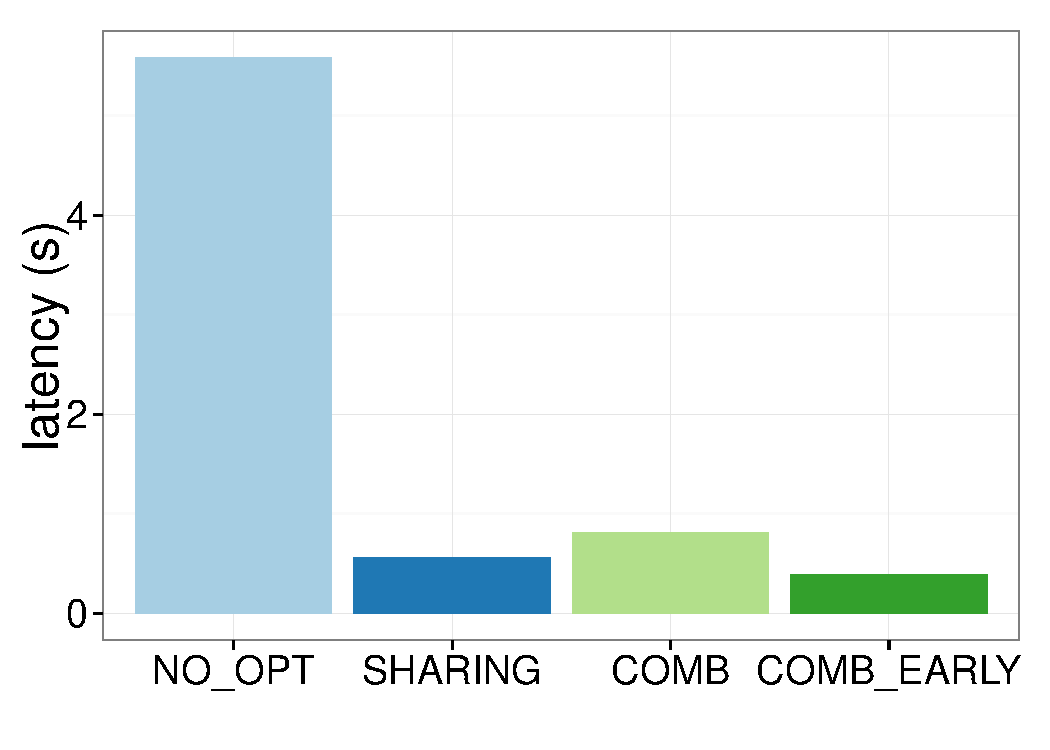
\includegraphics[width=3cm] {Images/all_opt_real_data_row_BANK.pdf}}
% 		\caption{BANK}
% 		\label{fig:baseline_size}
% 	\end{subfigure}
% 	\begin{subfigure}{0.24\linewidth}
% 		\centering
% 		{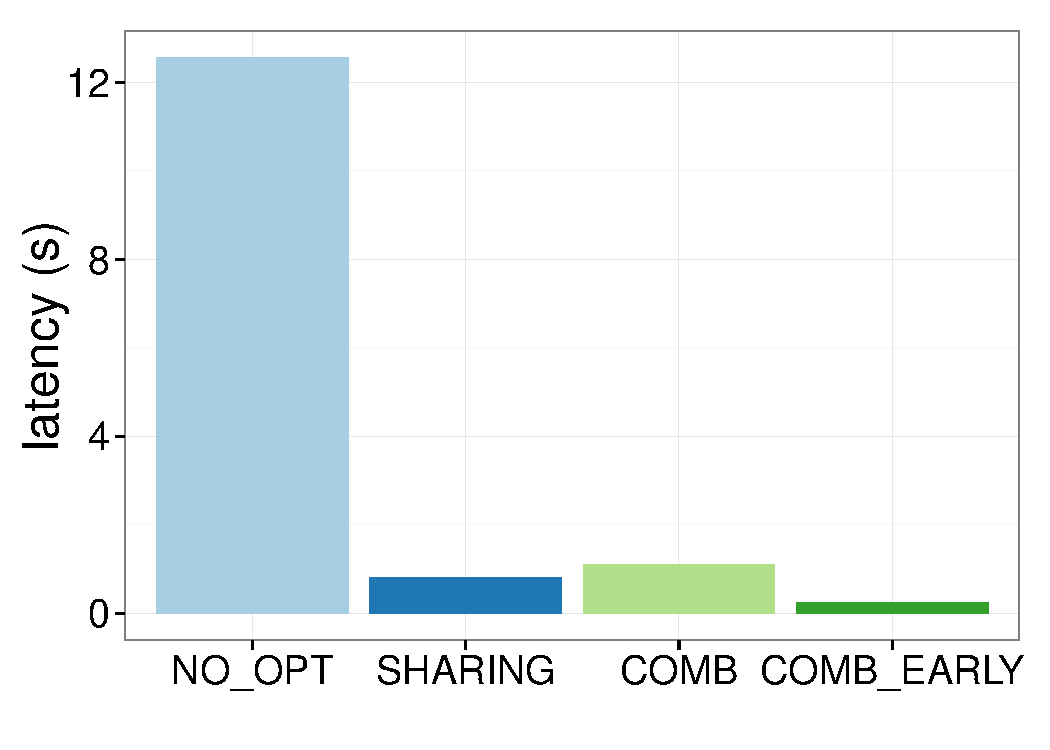
\includegraphics[width=3cm] {Images/all_opt_real_data_row_DIAB.pdf}}
% 		\caption{DIAB}
% 		\label{fig:baseline_views}
% 	\end{subfigure}
% 	\begin{subfigure}{0.24\linewidth}
% 		{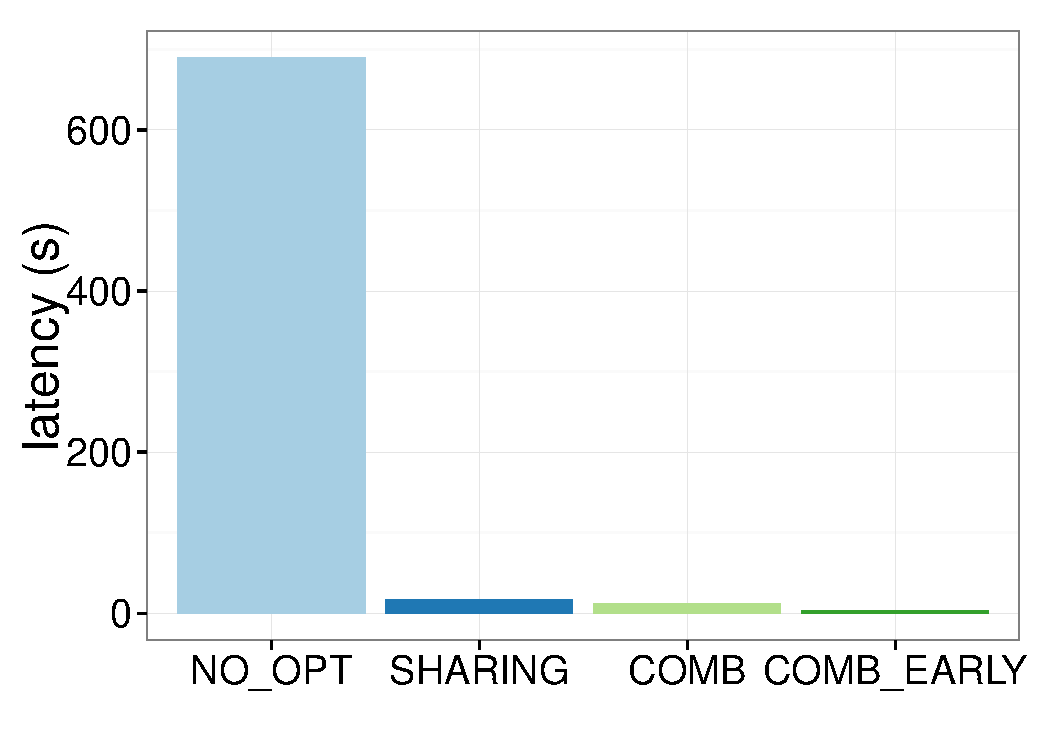
\includegraphics[width=3cm] {Images/all_opt_real_data_row_AIR.pdf}}
% 		\caption{AIR}
% 		\label{fig:multi_agg}
% 	\end{subfigure}
% 	\begin{subfigure}{0.24\linewidth}
% 		{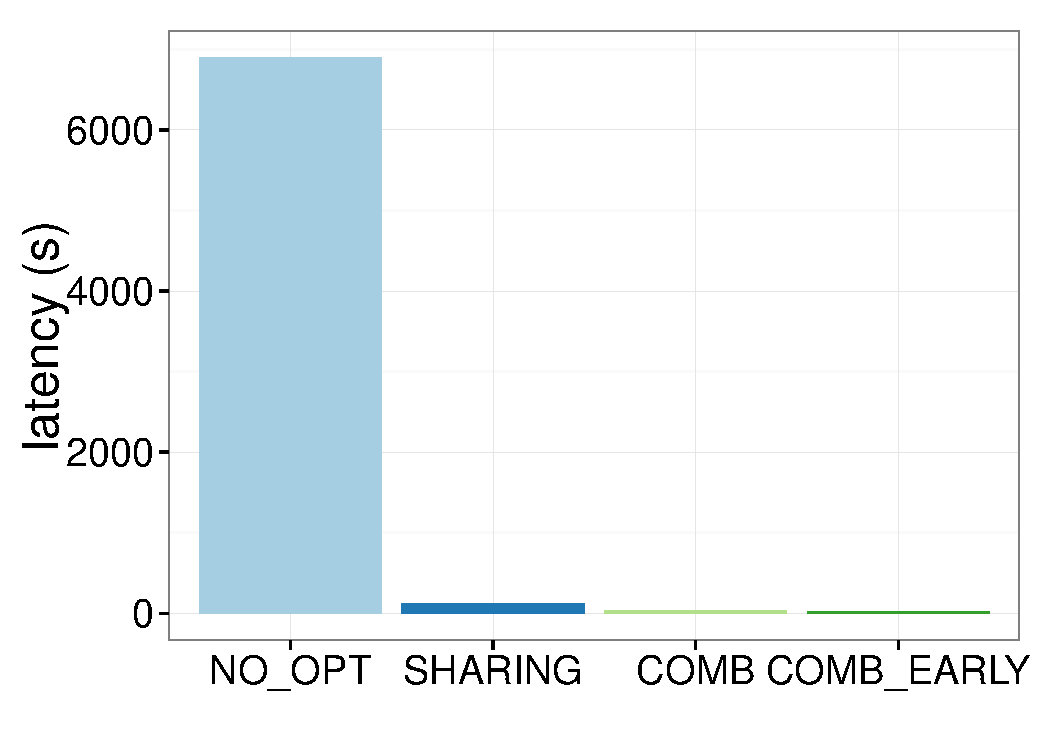
\includegraphics[width=3cm] {Images/all_opt_real_data_row_AIR10.pdf}}
% 		\caption{AIR10}
% 		\label{fig:multi_agg}
% 	\end{subfigure}
% 	\vspace{-10pt}
% 	\caption{Performance gains of all optimizations in ROW }
% 	\vspace{-10pt}
% 	\label{fig:share_prune_row}
% \end{figure}

\begin{figure}[h]
	\centering
	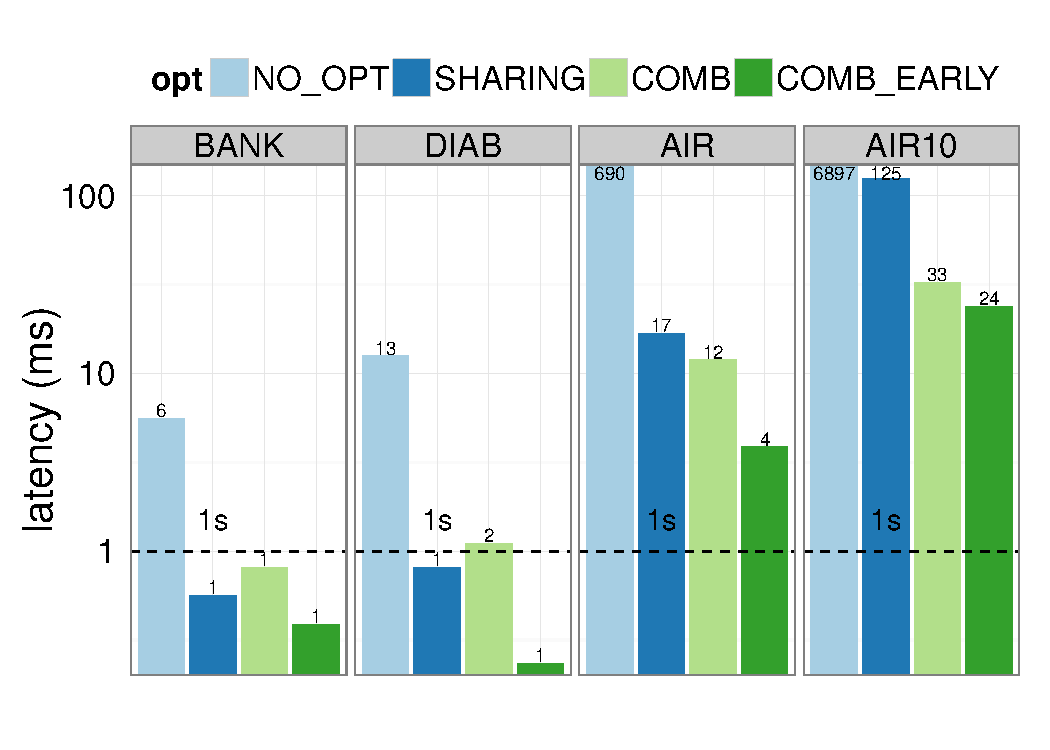
\includegraphics[width=9cm] {Images/all_opt_real_data_row.pdf}
	\caption{Performance gains of all optimizations in ROW}
	\label{fig:share_prune_row}
	\vspace{-15pt}
\end{figure}
 
\begin{denselist} 
\item The combination of our sharing and pruning optimizations provides a speedup of upto 50X (COMB) -- 150X (COMB\_EARLY) for ROW (shown above) and 40X (COMB) -- 80X (COMB\_EARLY) for COL (Section \ref{sec:sharing_and_pruning}).
This reduces latencies for small datasets like DIAB from 12s to 300ms, and from >1 hr to <30s for large datasets like AIR10.
\item The sharing optimizations (Section \ref{sec:sharing_opt}) alone produce performance gains of upto 40X for ROW and 10X for COL. This enables \SeeDB to process small and moderate sized datasets (1M rows, 100 views) in interactive time scales, i.e. within a few seconds.
\item Pruning optimizations (Section \ref{sec:in_memory_execution_engine}) provide additional gains of upto 5X. Early result return, in particular, enables real-time response for large datasets. E.g. for AIR, the EARLY strategy allows \SeeDB to return results in under 4s while processing the full dataset takes tens of seconds. We also find that quality of results is not adversely affected by pruning: the utility distance for all pruning strategies is close to 0.
\item In general, COL stores are better suited to the \SeeDB workload and outperform ROW stores. The column-oriented data layout of COL enables the selective processing of specific attributes involved in each visualization. 
\item Finally, while our techniques show performance gains across the board, they are particularly useful for large datasets, e.g. overall gain is much larger for AIR10 (150X) vs. BANK (10X). We also find that our SHARING optimization is best suited for small datasets like BANK and DIAB where pruning overhead degrades performance, while COMB and COMB\_EARLY are well suited for large datasets like AIR and AIR10.
\end{denselist}

In the next sections, we discuss the performance of individual optimizations and how they relate to the overall performance gain.



